%
% $RCSfile: looping.tex,v $
%
% Copyright (C) 2002-2008. Christian Heller.
%
% Permission is granted to copy, distribute and/or modify this document
% under the terms of the GNU Free Documentation License, Version 1.1 or
% any later version published by the Free Software Foundation; with no
% Invariant Sections, with no Front-Cover Texts and with no Back-Cover
% Texts. A copy of the license is included in the section entitled
% "GNU Free Documentation License".
%
% http://www.cybop.net
% - Cybernetics Oriented Programming -
%
% http://www.resmedicinae.org
% - Information in Medicine -
%
% Version: $Revision: 1.1 $ $Date: 2008-08-19 20:41:07 $ $Author: christian $
% Authors: Christian Heller <christian.heller@tuxtax.de>
%

\subsubsection{Looping}
\label{looping_heading}
\index{Looping}
\index{Loop Control Structure}
\index{Pre Test Loop}
\index{Post Test Loop}
\index{Counting Loop}
\index{while, while-do}
\index{do-while, repeat-until}
\index{for, for-next}

The \emph{Loop} (figure \ref{loop_figure}) is a control element that allows to
iterate through statements, in other words to execute them repeatedly, several
times. Its concept is quite simple -- a jump backwards in the program. However,
this low-level jump is hidden to the application programmer using a higher-level
SPP language. The loop is indicated by a special keyword instead, for example:

\begin{scriptsize}
    \begin{verbatim}
    while (condition) {
        statements;
    }
    \end{verbatim}
\end{scriptsize}

\begin{figure}[ht]
    \begin{center}
        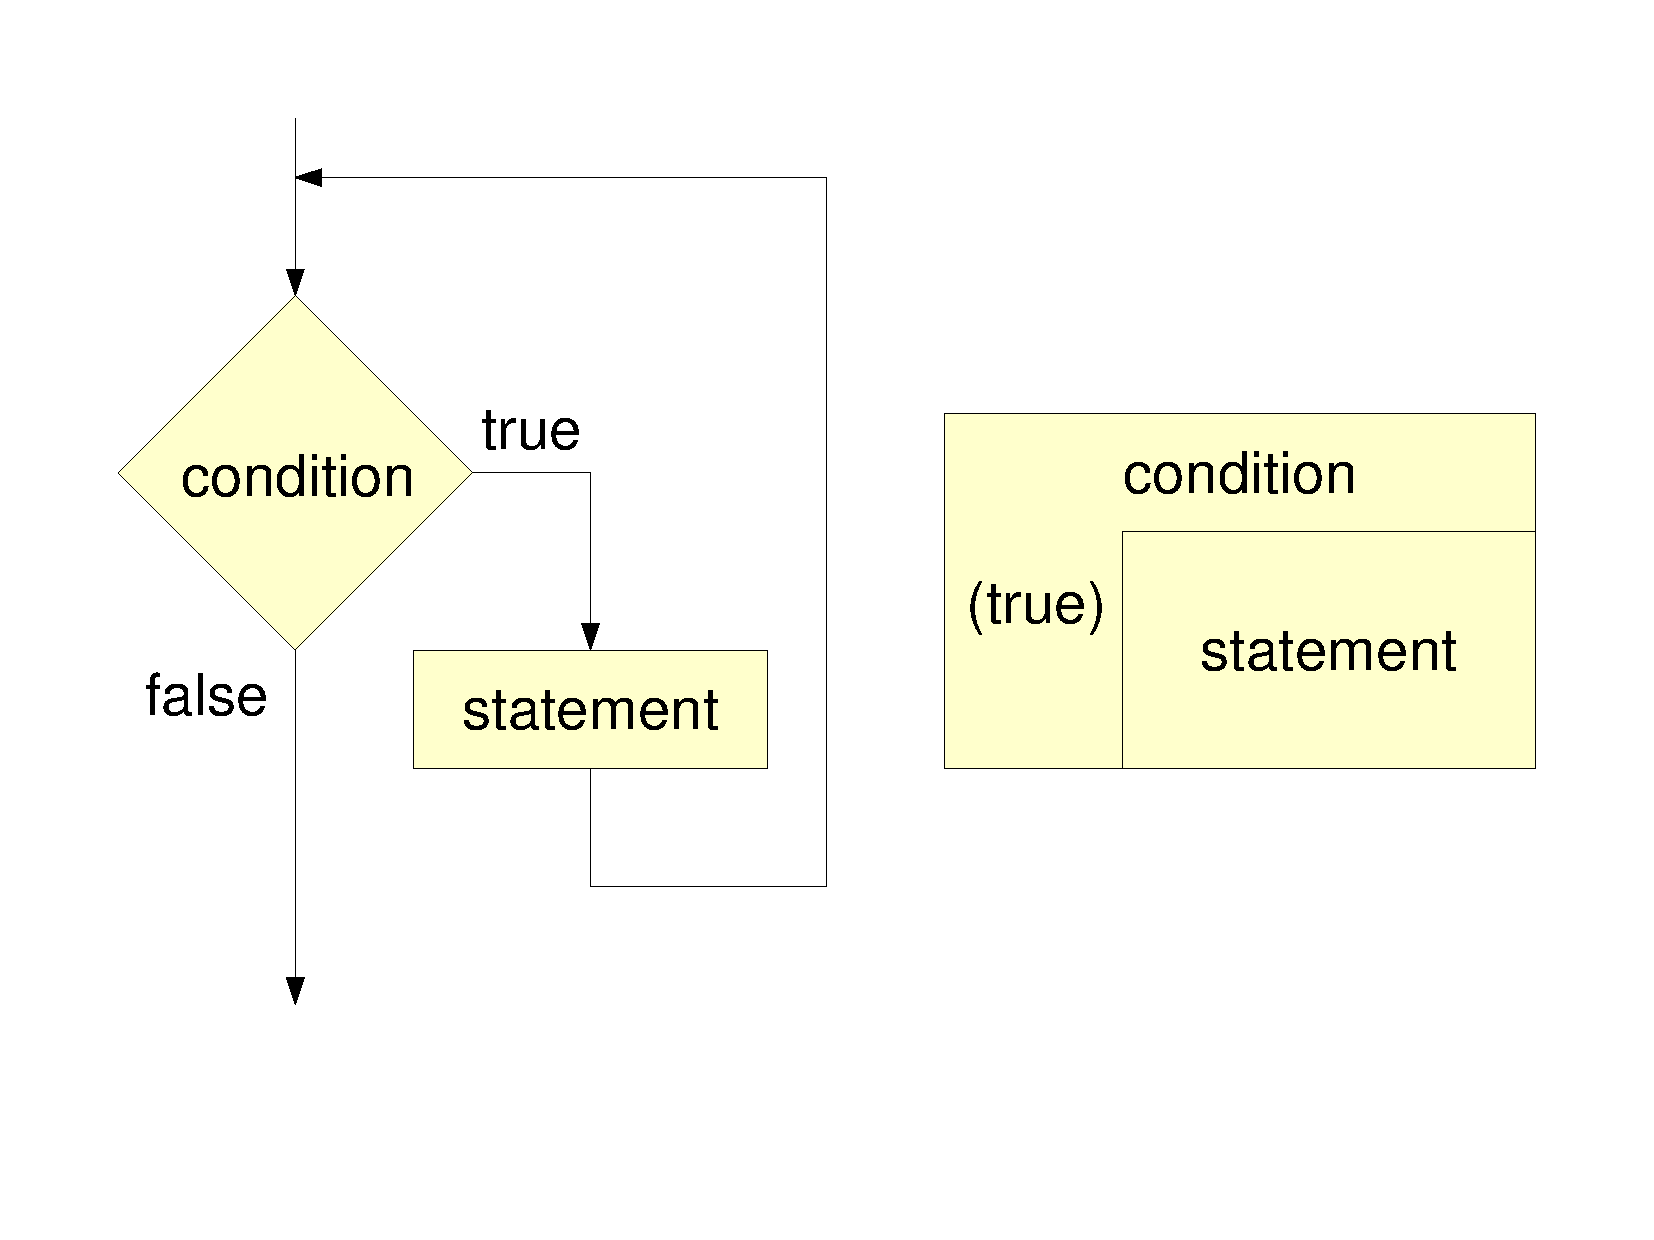
\includegraphics[scale=0.3,angle=-90]{graphic/loop.pdf}
        \caption{Loop as Program Flow Chart and Structure Chart}
        \label{loop_figure}
    \end{center}
\end{figure}

Most programming languages offer three different loop styles, as there are:

\begin{itemize}
    \item[-] Pre-test loop: \emph{while}, \emph{while-do}
    \item[-] Post-test loop: \emph{do-while}, \emph{repeat-until}
    \item[-] Counting Loop: \emph{for}, \emph{for-next}
\end{itemize}

A \emph{Pre-Test Loop} is used when one wants to check a condition before the
statements in the loop body are executed:

\begin{scriptsize}
    \begin{verbatim}
    int i = 0;
    while (i < 1) {
        statements;
        i++;
    }
    \end{verbatim}
\end{scriptsize}

The \emph{Post-Test Loop}, on the other hand, repeats all loop-body statements
until a condition is met:

\begin{scriptsize}
    \begin{verbatim}
    int i = 0;
    do {
        statements;
        i++;
    } while (i < 1);
    \end{verbatim}
\end{scriptsize}

A \emph{Counting Loop}, finally, can be applied when the number of necessary
repetitions of the loop-body statements is known in advance:

\begin{scriptsize}
    \begin{verbatim}
    int i;
    for (i = 0; i < 1; i++) {
        statements;
    }
    \end{verbatim}
\end{scriptsize}

The statements in all three loop examples are only executed once. It is not
difficult to see that the \emph{for} loop can be replaced with a \emph{while}
loop by initialising the \emph{i} variable in its declaration line and moving
the increment statement into the loop's block. But also the \emph{do-while}
loop can be replaced with a \emph{while} loop. If the behaviour does not match
(for example a while block is not executed even once), then changing the initial
loop variable value can solve this problem. Otherwise, modifying the statements
(algorithm) in the block, without changing it logically, will do.

As can be seen: Most variations of the \emph{Looping} concept are just a
convenience for the programmer. They are conceptually identical and can be lead
back to a simple loop with break condition, each. The interpreter described in
chapter \ref{cybernetics_oriented_interpreter_heading} uses just one kind of
loop.
